\documentclass[11pt,a4paper]{article}

% ── Packages ──────────────────────────────────────────────────────────
\usepackage[margin=1in]{geometry}
\usepackage{graphicx}
\usepackage{booktabs}
\usepackage{amsmath}
\usepackage{amssymb}
\usepackage{hyperref}
\usepackage{xcolor}
\usepackage{float}
\usepackage{caption}
\usepackage{subcaption}
\usepackage{enumitem}
\usepackage{fancyhdr}
\usepackage{titlesec}
\usepackage{multirow}

% ── Style ─────────────────────────────────────────────────────────────
\hypersetup{colorlinks=true, linkcolor=blue!60!black, citecolor=blue!60!black, urlcolor=blue!60!black}
\pagestyle{fancy}
\fancyhf{}
\fancyhead[L]{\small NL\_Hecate Experiment Report}
\fancyhead[R]{\small baseline\_pushup\_p2\_k2\_ext10k}
\fancyfoot[C]{\thepage}
\renewcommand{\headrulewidth}{0.4pt}

\definecolor{nlred}{HTML}{D84315}
\definecolor{nlgreen}{HTML}{2E7D32}
\definecolor{nlgray}{HTML}{616161}
\definecolor{nlorange}{HTML}{FF9800}
\titleformat{\section}{\Large\bfseries\color{nlred}}{}{0em}{}[\vspace{-0.5em}\rule{\textwidth}{0.4pt}]

% ══════════════════════════════════════════════════════════════════════
\begin{document}

% ── Title ─────────────────────────────────────────────────────────────
\begin{center}
    {\LARGE\bfseries Experiment Report: Push-Up k=2 Extension (+10K)}\\[0.6em]
    {\large\color{nlgray} NL\_Hecate --- Nested Learning Push-Up Pipeline}\\[0.4em]
    {\normalsize Run ID: \texttt{baseline\_pushup\_p2\_k2\_ext10k} \quad|\quad Date: 2026-03-15}\\[0.3em]
    {\normalsize GPU: A6000 (GPU\,0) \quad|\quad Duration: 2.3\,h \quad|\quad 609\,tok/s}\\[0.5em]
    {\large\color{red}\bfseries Outcome: CONFIRMED FAILURE --- Push-up k=2 initialization is ruled out}
\end{center}
\vspace{1em}

% ── Purpose ───────────────────────────────────────────────────────────
\section{Purpose}

The push-up $k{=}2$ experiment (report~2) showed regression across all metrics. This extension
tests whether \textbf{additional training time} resolves the problem. 10K more steps on fresh
data are added to the $k{=}2$ push-up's step-20K checkpoint.

\textbf{Hypothesis:} Given sufficient joint training, L0 and L1 will eventually differentiate and
the model will recover from the initial regression.

\textbf{Answer:} No. The levels remain trapped in a degenerate basin. The extension confirms
that the push-up initialization method is fundamentally flawed, not undertrained.

\textbf{Control:} A concurrent \textcolor{nlgreen}{fresh $k{=}2$ from random init} ran
on GPU\,1 for direct comparison. Results from this run (at step~10K) are included as contrast
throughout.


% ── Configuration ─────────────────────────────────────────────────────
\section{Configuration}

\begin{table}[H]
\centering
\caption{Extension run configuration. Only differences from the original push-up k=2 are shown.}
\label{tab:config}
\begin{tabular}{@{}lll@{}}
\toprule
\textbf{Parameter} & \textbf{Value} & \textbf{Change from p2\_k2} \\
\midrule
Steps              & 10{,}000 (20K$\to$30K total) & +10K extension \\
Donor checkpoint   & \texttt{baseline\_pushup\_p2\_k2/model.safetensors} & k=2 at 20K \\
Warmup steps       & 250 & Reduced (was 500) \\
Data seek          & 17{,}920{,}512 & 100\% fresh data \\
LR                 & $3 \times 10^{-4}$ cosine (re-started) & New cosine cycle \\
\midrule
\multicolumn{3}{@{}l@{}}{\textit{All other parameters identical: d=512, 4 blocks, k=2, chunk\_sizes=[1,8],}} \\
\multicolumn{3}{@{}l@{}}{\textit{m\_norm\_clamp disabled, TNT hierarchical, dolmino\_100b.}} \\
\bottomrule
\end{tabular}
\end{table}


% ── Results Summary ───────────────────────────────────────────────────
\section{Results Summary}

\begin{table}[H]
\centering
\caption{Key metrics at milestones (steps 20K--30K).}
\label{tab:milestones}
\begin{tabular}{@{}rrrrr@{}}
\toprule
\textbf{Step} & \textbf{Loss} & \textbf{PPL} & \textbf{Grad Norm} & \textbf{Block CV} \\
\midrule
20{,}000 & 3.935 & 51  & 2.10 & 0.328 \\
22{,}000 & 3.935 & 51  & 2.68 & 0.371 \\
24{,}000 & 5.582 & 266 & 3.84 & 0.269 \\
26{,}000 & 2.838 & 17  & 2.03 & 0.303 \\
28{,}000 & 3.214 & 25  & 2.09 & 0.296 \\
30{,}000 & 2.906 & 18  & 2.82 & 0.329 \\
\bottomrule
\end{tabular}
\end{table}

\begin{table}[H]
\centering
\caption{Smoothed loss trajectory (50-step windows).}
\label{tab:trajectory}
\begin{tabular}{@{}lcc@{}}
\toprule
\textbf{Window} & \textbf{Mean Loss} & \textbf{Mean Grad Norm} \\
\midrule
Steps 20K--21K & 3.458 & 2.254 \\
Steps 22K--23K & 3.444 & 2.403 \\
Steps 24K--25K & 3.312 & 2.193 \\
Steps 26K--27K & 3.391 & 2.234 \\
Steps 28K--29K & 3.297 & 2.367 \\
Steps 29K--30K & 3.276 & 2.255 \\
\bottomrule
\end{tabular}
\end{table}

\noindent \textbf{Summary:} Loss improved marginally (3.46 $\to$ 3.28 mean), still well above the
$k{=}1$ baseline (2.84) and the fresh $k{=}2$ trajectory (3.70 at step~10K, trending down).
The 10K extension bought almost nothing.


% ── All-Experiment Loss ──────────────────────────────────────────────
\section{Loss: Full Experimental Context}

\begin{figure}[H]
    \centering
    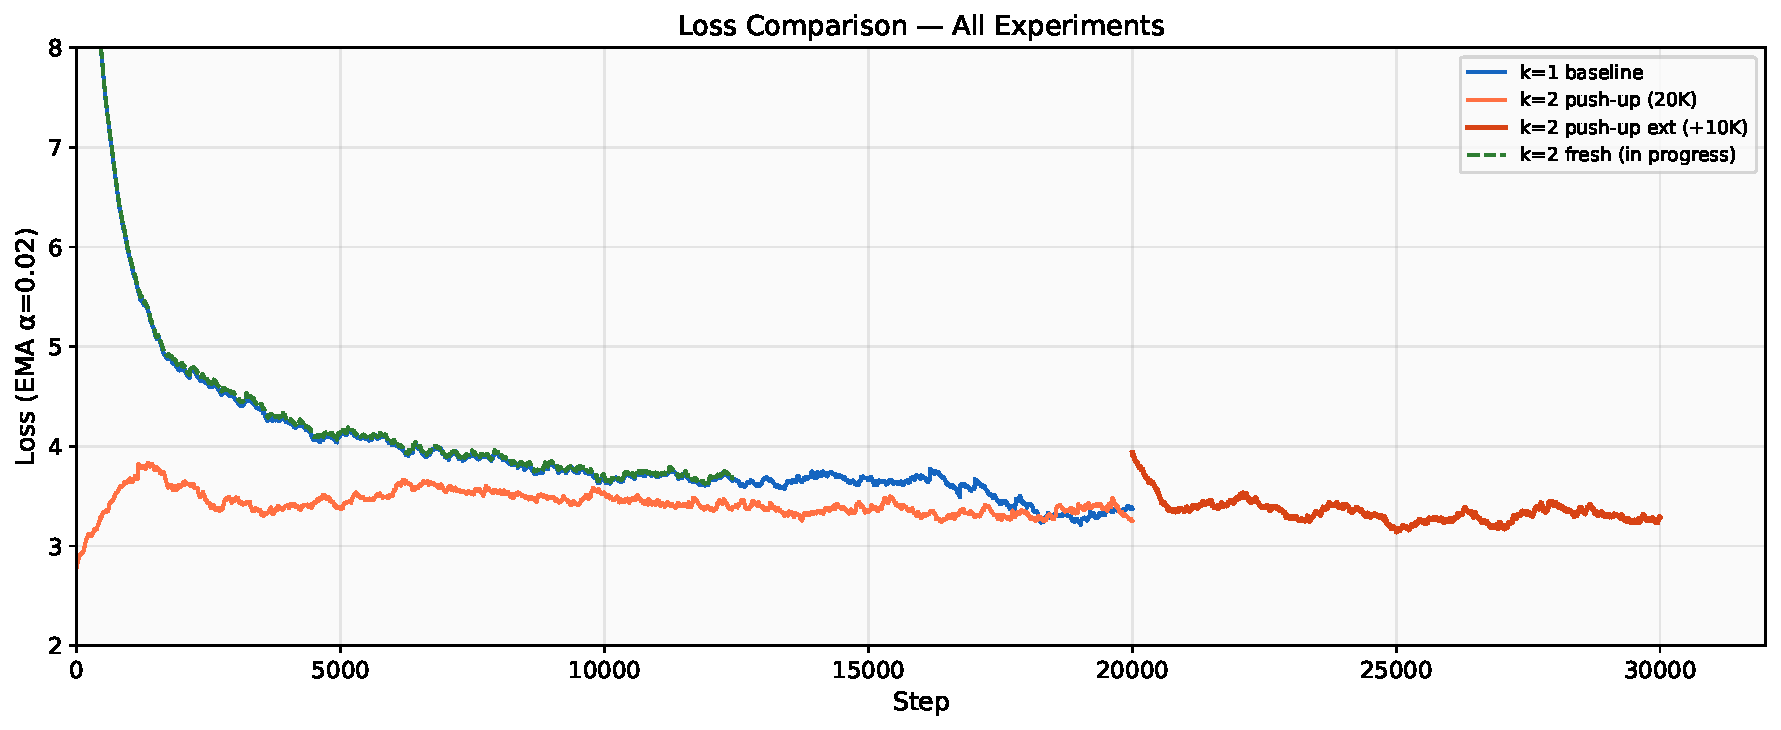
\includegraphics[width=\textwidth]{fig_loss_all.pdf}
    \caption{Loss comparison across all four experiments. The extension (dark red) continues
    the push-up's plateau from steps 20K--30K. The fresh k=2 (green dashed) is already
    converging faster from random init.}
    \label{fig:loss_all}
\end{figure}

The four-experiment overlay tells the complete story:
\begin{itemize}[topsep=4pt, itemsep=2pt]
    \item \textbf{k=1 baseline} (blue): Converges to 2.84 at step 20K.
    \item \textbf{Push-up k=2} (orange): Regresses from 2.79, plateaus at $\sim$3.4.
    \item \textbf{Push-up ext +10K} (dark red): Continues the same plateau, ending at $\sim$3.28.
    \item \textbf{Fresh k=2} (green): Starts at 11.0, reaches 3.70 at step 10K with a steeper
    descent slope. Projected to reach $\sim$3.0 by step 20K.
\end{itemize}

\noindent The push-up spent 30{,}000 total steps (20K + 10K extension) to reach a loss of 3.28.
The fresh k=2 will likely beat that in under 15K steps from random init. More training cannot
fix a broken initialization.


% ── Loss Detail ──────────────────────────────────────────────────────
\begin{figure}[H]
    \centering
    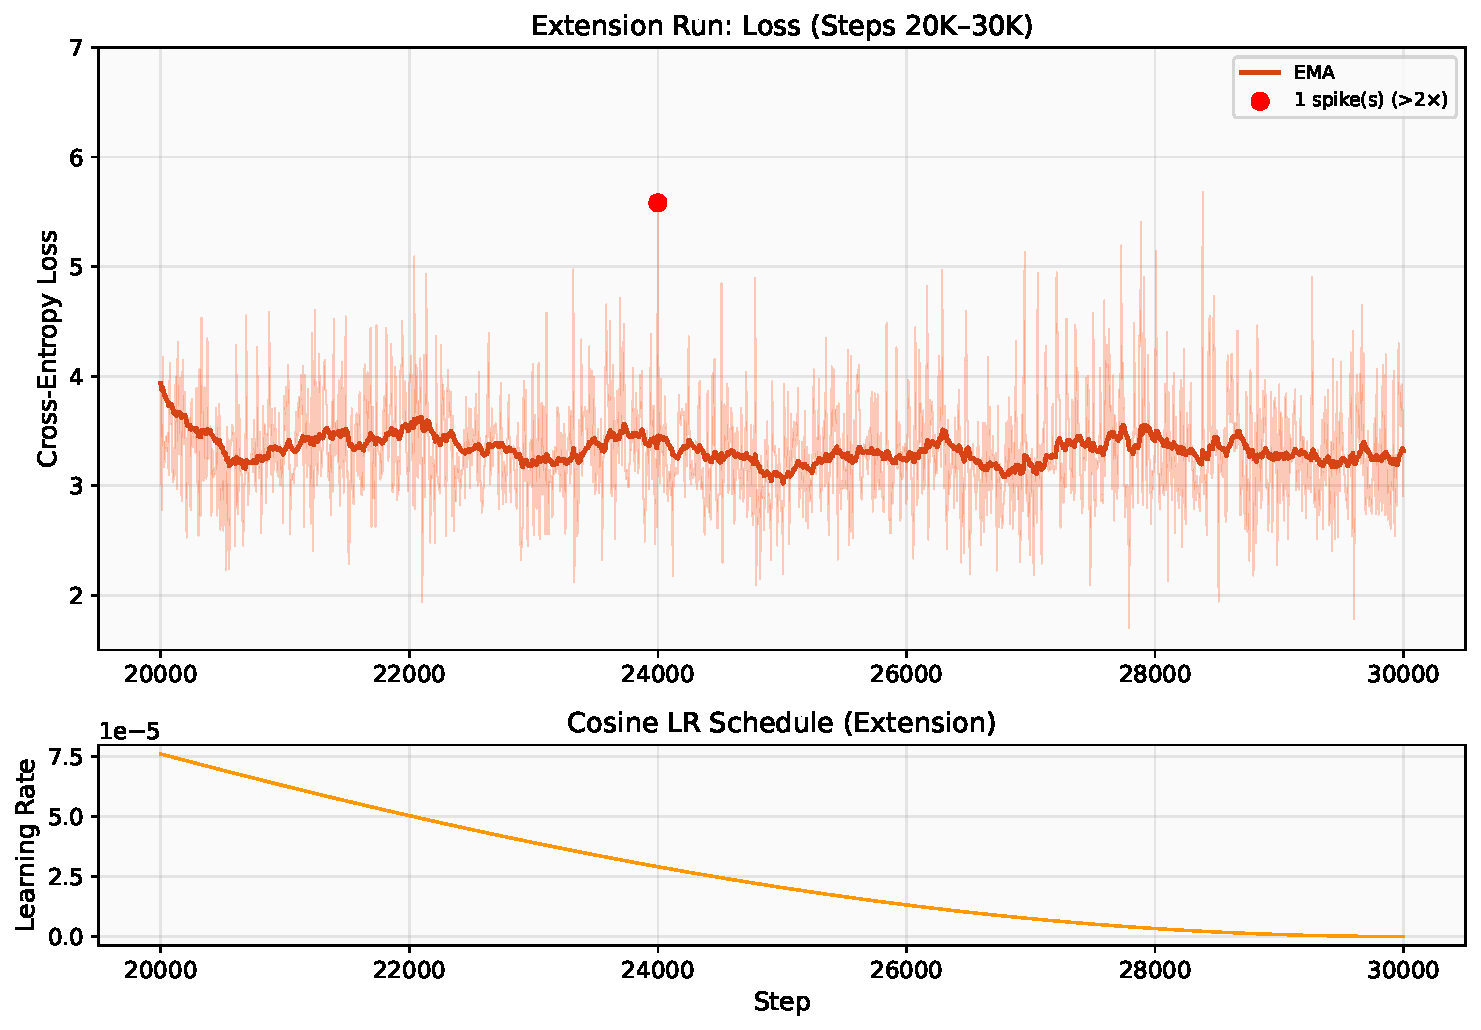
\includegraphics[width=\textwidth]{fig_loss_ext.pdf}
    \caption{Extension run loss detail. One major spike at step 24K (loss=5.58)
    correlates with L1 theta instability (see Section~\ref{sec:theta}).}
    \label{fig:loss_ext}
\end{figure}


% ── Gradient Analysis ─────────────────────────────────────────────────
\section{Gradient Analysis}

\begin{figure}[H]
    \centering
    
\includegraphics[width=\textwidth]{fig_grad_norms.pdf}
    \caption{Per-block gradient norms and CV during the extension.
    CV hovers at $\sim$0.30, below the 0.3 threshold for meaningful specialization.}
    \label{fig:gnorms}
\end{figure}

\begin{figure}[H]
    \centering
    
\includegraphics[width=\textwidth]{fig_l0_gnorms.pdf}
    \caption{L0 inner-loop gradient norms. Block~0 dominates ($\sim$0.35) but no growth
    trend is visible --- the memory mechanism has stagnated.}
    \label{fig:l0}
\end{figure}


% ══════════════════════════════════════════════════════════════════════
% GATE DIAGNOSTICS — the core of this report
% ══════════════════════════════════════════════════════════════════════
\section{Gate Diagnostics: The Oscillation Problem}
\label{sec:theta}

This section presents the tape-level diagnostics that explain \textbf{why} the push-up fails.
The extension run logged 20 tape snapshots with per-level gate statistics (alpha, theta, eta)
for every block. A concurrent fresh $k{=}2$ run provides the control comparison.


% ── Theta ─────────────────────────────────────────────────────────────
\subsection{Theta (Inner-Loop Learning Rate): Oscillation vs Convergence}

\begin{figure}[H]
    \centering
    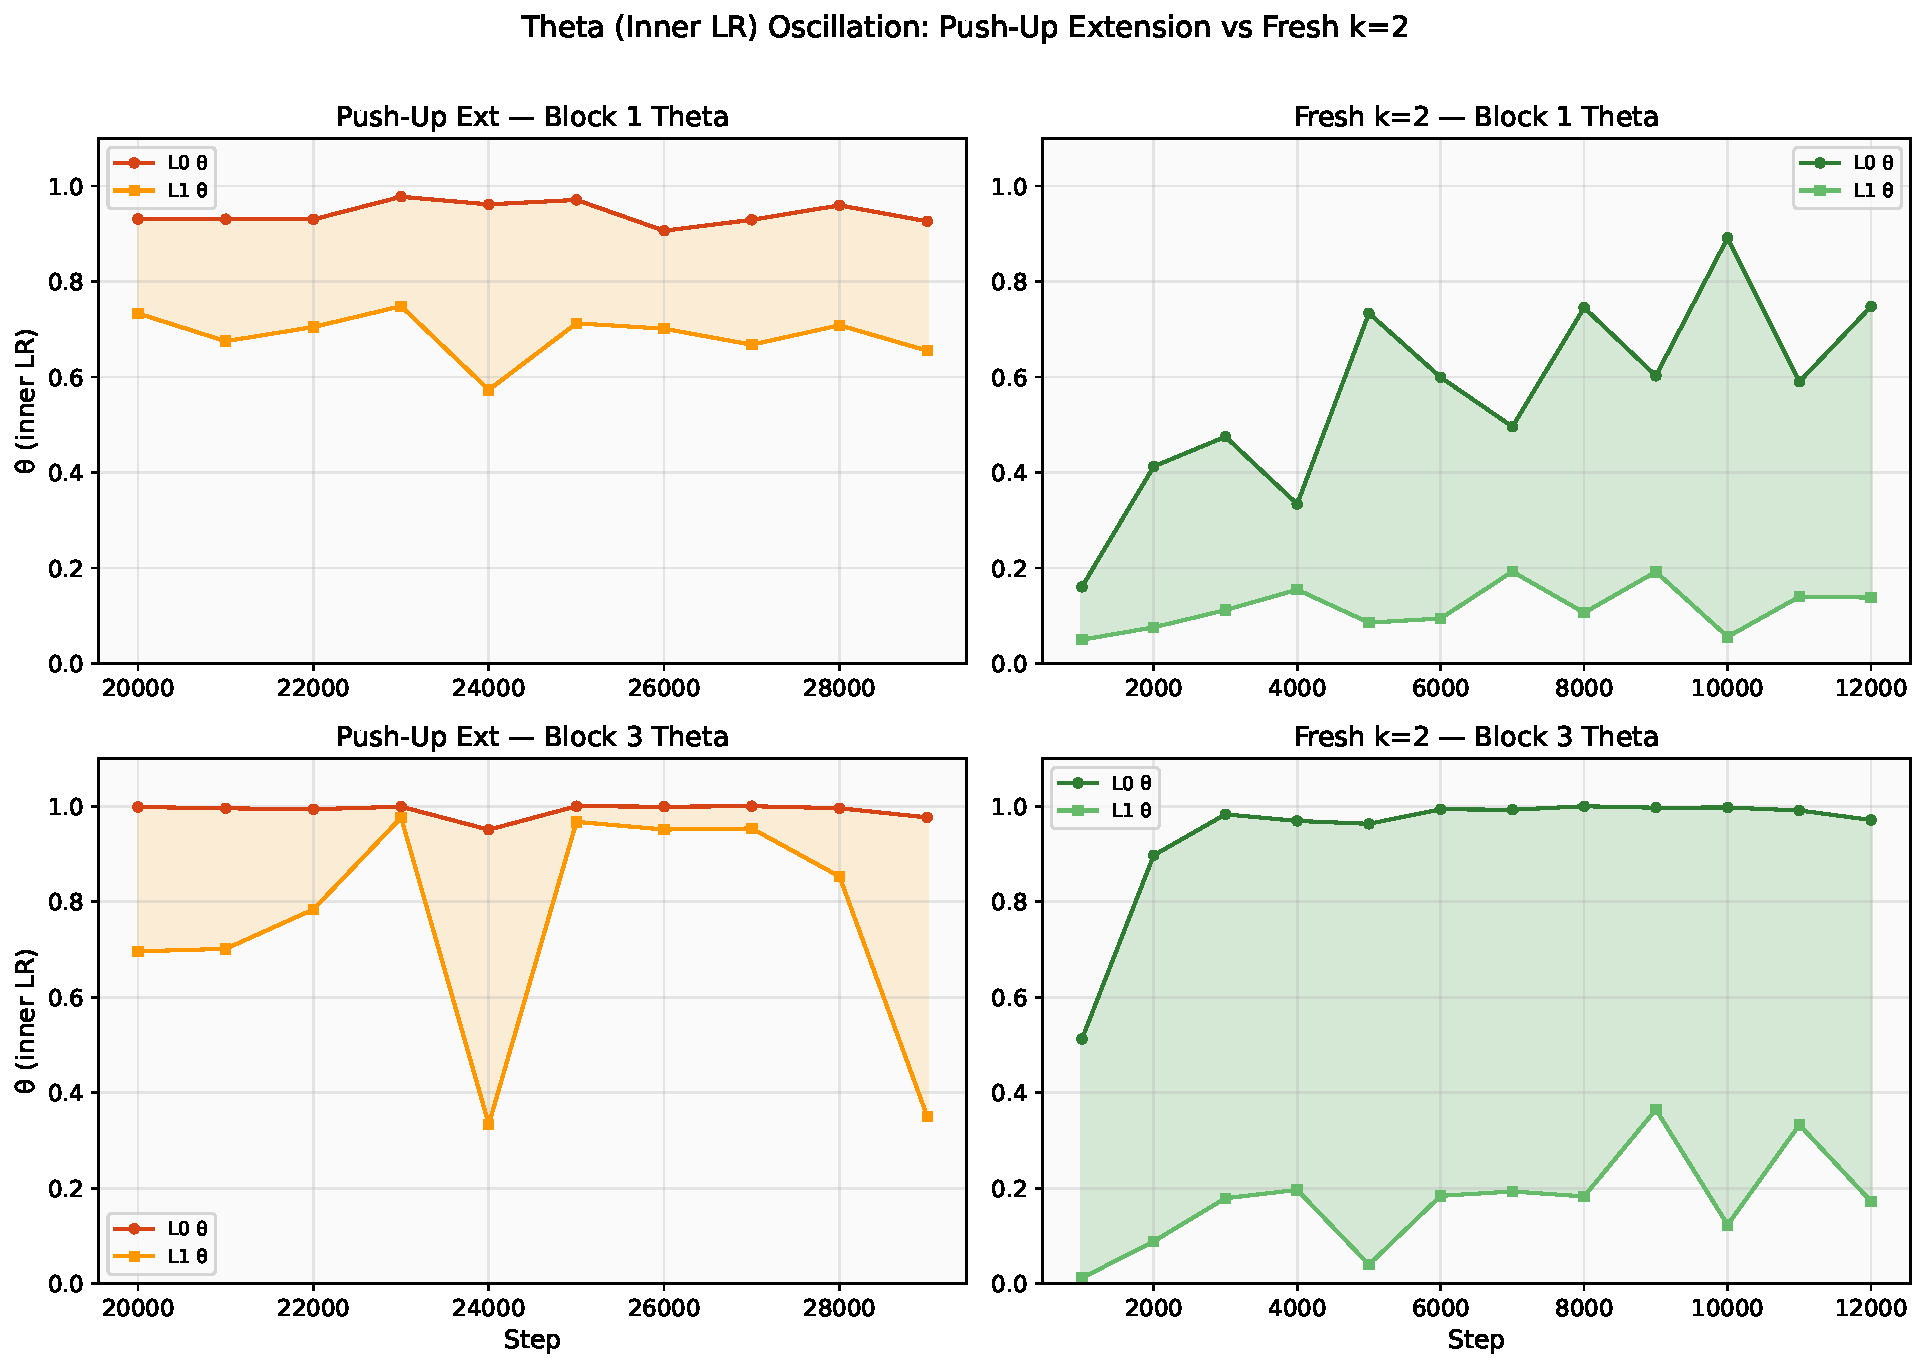
\includegraphics[width=\textwidth]{fig_theta_comparison.pdf}
    \caption{Theta (inner-loop LR) for L0 and L1 across two blocks. \textbf{Left:} Push-up
    extension --- L1 theta oscillates wildly, especially in Block~3.
    \textbf{Right:} Fresh k=2 --- L0 rises to $\sim$0.9, L1 stays low ($<$0.2).
    Shaded area shows L0-L1 gap.}
    \label{fig:theta}
\end{figure}

\begin{table}[H]
\centering
\caption{Block~3 L1 theta: push-up extension showing extreme oscillation.}
\label{tab:theta_osc}
\begin{tabular}{@{}rccl@{}}
\toprule
\textbf{Step} & \textbf{L0 $\theta$} & \textbf{L1 $\theta$} & \textbf{Behavior} \\
\midrule
20{,}000 & 0.998 & 0.696 & Moderate \\
23{,}000 & 0.999 & \textbf{0.976} & Rockets to ceiling \\
24{,}000 & 0.951 & \textcolor{red}{\textbf{0.334}} & Crashes (loss spike) \\
25{,}000 & 1.000 & \textbf{0.967} & Rockets back up \\
28{,}000 & 0.996 & 0.853 & Partial recovery \\
29{,}000 & 0.977 & \textcolor{red}{\textbf{0.351}} & Crashes again \\
\bottomrule
\end{tabular}
\end{table}

\noindent L1 theta in Block~3 exhibits \textbf{0.6+ swings} between adjacent tape snapshots.
It oscillates between ``maximally aggressive'' ($\sim$0.97) and ``nearly shut off'' ($\sim$0.33)
with no convergence over 10K steps. L0 theta, inherited from $k{=}1$ training, remains pinned
at the ceiling ($>$0.95) with no room to modulate.

In contrast, the fresh $k{=}2$ shows clean separation: L0 rises to $\sim$0.99 while L1 stays
below 0.2 throughout. Each level has found a distinct, stable role.

\textbf{The step-24K loss spike (5.58) directly correlates with L1 theta crashing to 0.334.}
When L1 abruptly changes its inner-loop learning rate by $3\times$, the forward pass geometry
shifts and the model produces incoherent outputs.


% ── Alpha ─────────────────────────────────────────────────────────────
\subsection{Alpha (Retention): No Timescale Separation}

\begin{figure}[H]
    \centering
    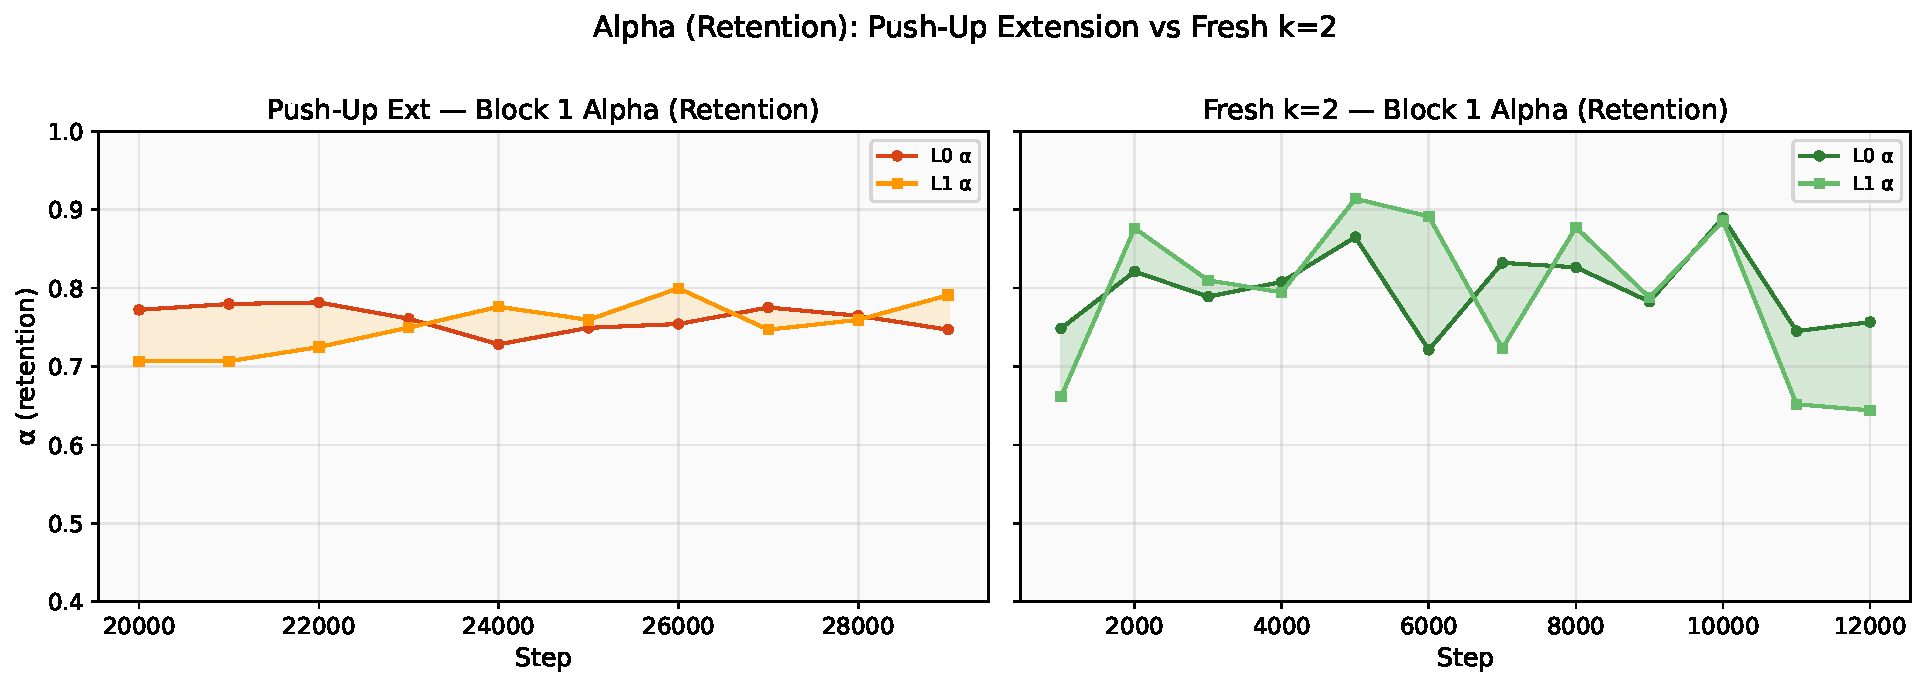
\includegraphics[width=\textwidth]{fig_alpha_comparison.pdf}
    \caption{Alpha (retention) for Block~1. \textbf{Left:} Push-up extension --- L0 and L1
    alpha overlap with no separation trend. \textbf{Right:} Fresh k=2 --- alpha values
    cross and wander but show slightly more range.}
    \label{fig:alpha}
\end{figure}

Alpha presents the weakest differentiation signal in \emph{both} experiments:
\begin{itemize}[topsep=4pt, itemsep=2pt]
    \item \textbf{Push-up ext:} L0 alpha $\approx$ 0.75, L1 alpha $\approx$ 0.75. Delta oscillates
    $\pm$0.05 with no trend. The levels have identical retention --- no memory timescale separation.
    \item \textbf{Fresh k=2:} L0 alpha $\approx$ 0.80, L1 alpha $\approx$ 0.82. Slightly wider
    range but still largely overlapping. Occasional excursions to $-$0.17 delta suggest the
    potential for separation, but it has not stabilized by step 10K.
\end{itemize}

\noindent \textbf{This motivates the retention initialization experiment}: if alpha=0.8 produces
minimal separation, starting at alpha=0.5 (maximum freedom to move in either direction) may
allow the model to discover distinct retention rates per level.


% ── Eta ───────────────────────────────────────────────────────────────
\subsection{Eta (Output Gate): Moderate Separation}

\begin{figure}[H]
    \centering
    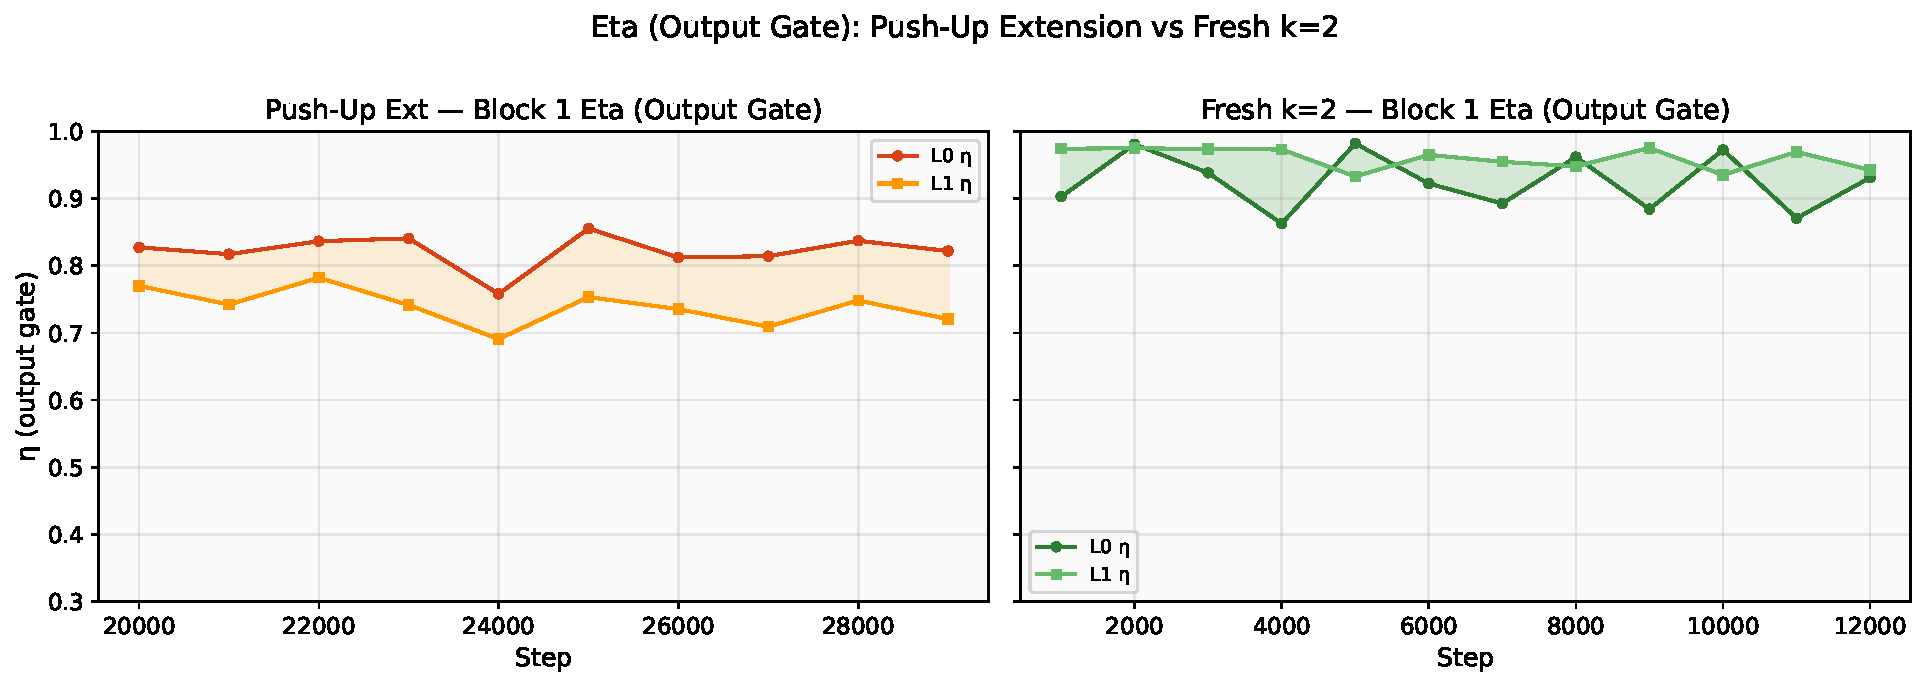
\includegraphics[width=\textwidth]{fig_eta_comparison.pdf}
    \caption{Eta (output gate) for Block~1. Both experiments show L0 eta $>$ L1 eta,
    with the fresh k=2 exhibiting wider separation.}
    \label{fig:eta}
\end{figure}

Eta shows the most consistent differentiation of the three gates:
\begin{itemize}[topsep=4pt, itemsep=2pt]
    \item \textbf{Push-up ext:} L0 eta $\approx$ 0.83, L1 eta $\approx$ 0.74. Gap $\sim$0.09.
    \item \textbf{Fresh k=2:} L0 eta starts higher and L1 lower, with gap $\sim$0.10--0.15.
\end{itemize}

\noindent L0 contributes more to the output than L1 in both experiments, which is consistent
with L0 firing every token (more data, more confident) while L1 fires every 8th.


% ── DGD Ratio ─────────────────────────────────────────────────────────
\subsection{DGD Update Magnitude Ratio}

\begin{figure}[H]
    \centering
    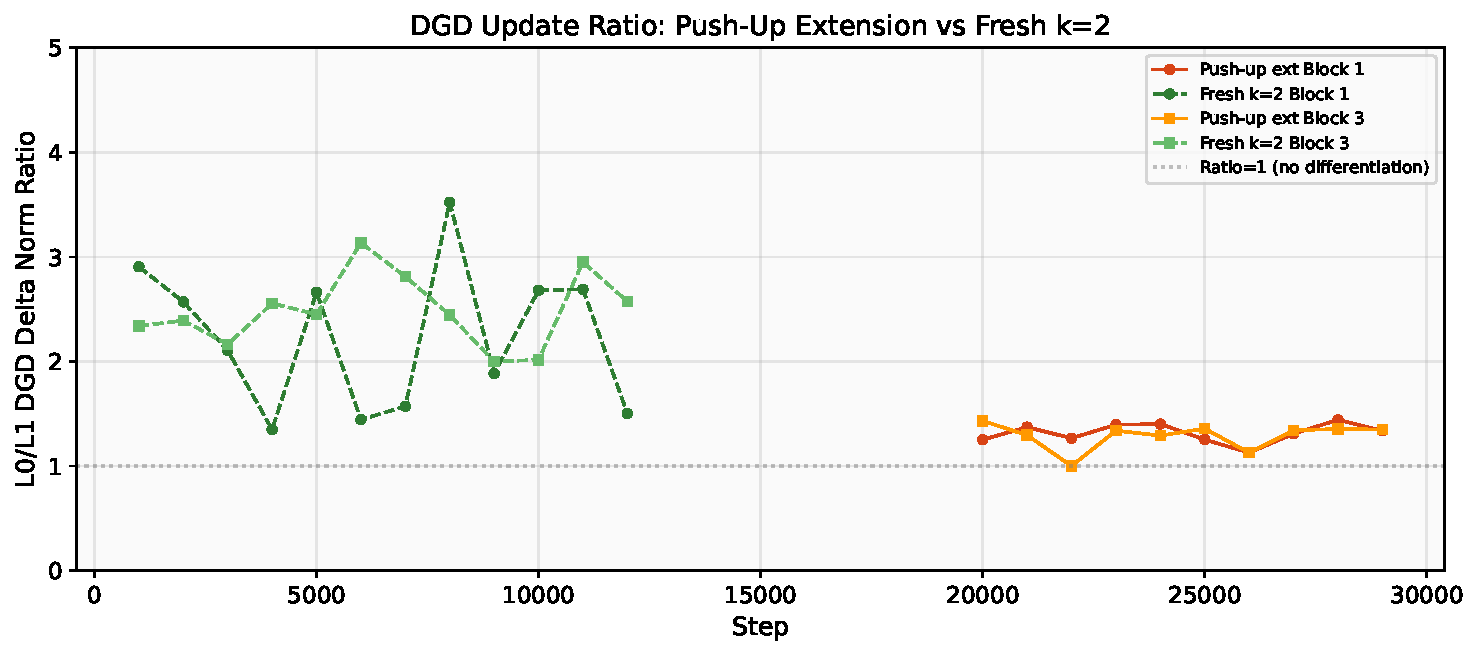
\includegraphics[width=\textwidth]{fig_dgd_ratio.pdf}
    \caption{L0/L1 DGD delta norm ratio. Push-up ext (circles) is stuck at $\sim$1.3.
    Fresh k=2 (squares) reaches 2.5--3.5 --- L0 makes much larger memory updates.}
    \label{fig:dgd}
\end{figure}

The DGD ratio measures how much larger L0's memory updates are compared to L1's.
\begin{itemize}[topsep=4pt, itemsep=2pt]
    \item \textbf{Push-up ext:} Stuck at 1.1--1.4 for the entire 10K extension. No growth.
    \item \textbf{Fresh k=2:} Ranges from 1.4 to 3.5, with higher values as training progresses.
    L0 is making 2--3$\times$ larger updates, consistent with its 8$\times$ higher firing rate.
\end{itemize}

\noindent A healthy DGD ratio $>$2 means the levels are making updates of different magnitudes,
which is a necessary condition for them to learn distinct representations.


% ── Output Grad Norms ─────────────────────────────────────────────────
\subsection{Output Gradient Norms: Identical in Both Experiments}

\begin{figure}[H]
    \centering
    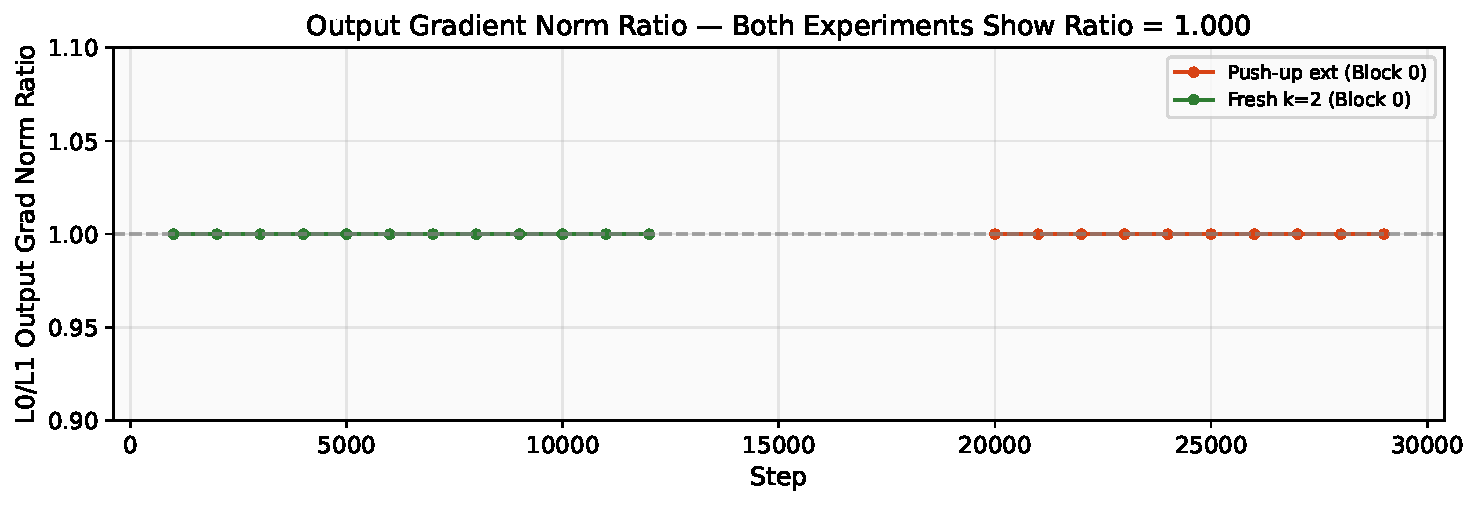
\includegraphics[width=\textwidth]{fig_outgrad_ratio.pdf}
    \caption{L0/L1 output gradient norm ratio = 1.000 in both experiments.
    This is a structural property of MAG composition, not a bug.}
    \label{fig:outgrad}
\end{figure}

The output gradient norm ratio is \textbf{exactly 1.000} across all snapshots in both experiments.
L0 and L1 receive identical gradient signals from the loss. This is a structural property of the
MAG (memory-attention-gated) composition: both levels contribute to a single gated sum, so the
backward pass distributes the same gradient to both.

\textbf{Implication:} Level differentiation cannot come from the output gradient. It must come
entirely from:
\begin{enumerate}[topsep=4pt, itemsep=2pt]
    \item The \textbf{frequency gap} (8$\times$) --- L0 fires every token, L1 every 8th
    \item The \textbf{inner-loop gate gradients} --- alpha, theta, eta are per-level learnable
    \item The \textbf{DGD update magnitude} --- different because of accumulated inner-loop state
\end{enumerate}

The fresh $k{=}2$ achieves differentiation through pathways 1--3 despite identical output
gradients. The push-up cannot because the cloned initialization neutralizes all three pathways.


% ── Throughput ────────────────────────────────────────────────────────
\section{Training Throughput}

\begin{figure}[H]
    \centering
    
\includegraphics[width=\textwidth]{fig_throughput.pdf}
    \caption{Extension run throughput: stable at 609~tok/s.}
    \label{fig:throughput}
\end{figure}


% ── Root Cause ────────────────────────────────────────────────────────
\section{Root Cause: Cloned Initialization Traps Both Levels}

The extension confirms the diagnosis from the push-up report (report~2), with additional
gate-level evidence:

\begin{enumerate}[topsep=4pt, itemsep=2pt]
    \item \textbf{L0 theta saturated at ceiling} ($>$0.95) --- inherited from $k{=}1$, cannot adapt.
    \item \textbf{L1 theta oscillating} (0.33 $\leftrightarrow$ 0.97) --- no stable equilibrium
    exists because L1 receives the same gradient as L0.
    \item \textbf{Alpha undifferentiated} ($\Delta \approx \pm 0.05$) --- no memory timescale
    separation. Both levels retain at the same rate.
    \item \textbf{DGD ratio stuck at $\sim$1.3} --- both levels make nearly identical magnitude
    updates, preventing representation divergence.
    \item \textbf{Output gradients identical} (ratio = 1.000) --- differentiation pressure comes
    only from frequency gap and inner-loop gates.
    \item \textbf{10K more steps did not help} --- this is a basin problem, not a budget problem.
\end{enumerate}

\noindent The push-up clones a converged single-level model into two copies. Both start
in the same optimization basin with identical weights, identical gates, and identical gradients.
The 8$\times$ frequency gap is insufficient pressure to break this symmetry when the
initialization is degenerate.


% ── Fresh k=2 Contrast ───────────────────────────────────────────────
\section{Control: Fresh k=2 (Concurrent Run)}

\begin{table}[H]
\centering
\caption{Push-up ext (step 27K) vs fresh k=2 (step 10K) gate diagnostics.}
\label{tab:comparison}
\begin{tabular}{@{}lccc@{}}
\toprule
\textbf{Metric} & \textbf{Push-Up Ext} & \textbf{Fresh k=2} & \textbf{Verdict} \\
\midrule
L0-L1 theta delta (Blk 1) & +0.20 to +0.27 & \textcolor{nlgreen}{\textbf{+0.64 to +0.84}} & Fresh 3$\times$ wider \\
L1 theta stability (Blk 3) & 0.33--0.98 & \textcolor{nlgreen}{\textbf{0.01--0.36}} & Fresh stable \\
L0-L1 alpha delta & $\pm$0.05 & $\pm$0.17 & Both weak \\
DGD ratio (Blk 1) & 1.1--1.4 & \textcolor{nlgreen}{\textbf{1.4--3.5}} & Fresh 2$\times$ higher \\
Block CV & 0.27--0.37 & \textcolor{nlgreen}{\textbf{0.40--0.58}} & Fresh more specialized \\
Loss spikes ($>$2$\times$) & 1 in 10K & \textcolor{nlgreen}{\textbf{0 in 10K}} & Fresh stable \\
\bottomrule
\end{tabular}
\end{table}

\noindent The fresh $k{=}2$ achieved stronger differentiation in \textbf{2K steps} than the
push-up achieved in \textbf{30K steps}. Every gate diagnostic favors fresh initialization.


% ── Conclusions ───────────────────────────────────────────────────────
\section{Conclusions}

\subsection{Verdict}

The $k{=}1 \to k{=}2$ push-up initialization method is \textbf{ruled out}. The 10K extension
confirmed that additional training does not resolve the differentiation failure. The levels are
trapped in the same optimization basin and cannot escape.

\subsection{Key Findings}

\begin{enumerate}[topsep=4pt, itemsep=2pt]
    \item \textbf{Theta oscillation is the proximal failure mode.} L1 theta bounces 0.6+ between
    snapshots because it receives the same gradient as L0 but is trying to find a different role.
    The oscillation directly causes loss spikes.

    \item \textbf{Alpha never separated.} Neither experiment produced strong retention-rate
    differentiation at alpha=0.8. This is the motivation for the retention=0.5 experiment:
    test whether alpha is learnable from a neutral starting point.

    \item \textbf{Output gradient identity is structural.} Both levels will always receive the same
    output gradient under MAG composition. Differentiation must come from frequency, gates,
    and inner-loop dynamics alone.

    \item \textbf{Fresh initialization works.} The concurrent fresh $k{=}2$ proves that two
    levels \emph{can} self-organize from random init. The 8$\times$ frequency gap provides
    sufficient structural pressure when the initialization is not degenerate.
\end{enumerate}

\subsection{Implications for the Push-Up Pipeline}

The push-up strategy is not invalidated --- it is \textbf{reframed}. The correct approach
builds from the foundation up:

\begin{enumerate}[topsep=4pt, itemsep=2pt]
    \item \textbf{Fresh $k{=}2$}: Train the two slowest levels (L2, L3) from random init until
    differentiated and converged. These become the anchor.

    \item \textbf{Push-up two levels}: Add L0 and L1 simultaneously on top of the established
    L2/L3. The new levels are a matched pair with the same 8$\times$ ratio that already proved
    viable in the fresh $k{=}2$ run. L1 meshes with L2 at 8$\times$; L0 meshes with L1 at
    8$\times$. The gear train self-assembles.

    \item \textbf{Retention initialization}: Use the results of the retention=0.5 experiment
    to determine whether new levels should start with neutral retention (0.5) or need a floor
    until the inter-level relationship stabilizes.
\end{enumerate}

\subsection{Next Experiments}

\begin{enumerate}[topsep=4pt, itemsep=2pt]
    \item \textbf{Complete fresh $k{=}2$ (GPU\,1)} --- confirm differentiation holds to 20K.
    \item \textbf{Retention=0.5 probe (10K)} --- does the model set its own retention rate?
    \item \textbf{If successful, extend to 50K} --- two comparison points (0.5 vs 0.8 retention).
    \item \textbf{Two-level push-up $k{=}2 \to k{=}4$} --- the real test of the gear-train
    hypothesis, using the best $k{=}2$ donor.
\end{enumerate}

\end{document}
